% !TeX program = pdfLaTeX
\documentclass[12pt]{article}
\usepackage{amsmath}
\usepackage{graphicx,psfrag,epsf}
\usepackage{enumerate}
\usepackage{natbib}
\usepackage{textcomp}
\usepackage[hyphens]{url} % not crucial - just used below for the URL
\usepackage{hyperref}

%\pdfminorversion=4
% NOTE: To produce blinded version, replace "0" with "1" below.
\newcommand{\blind}{0}

% DON'T change margins - should be 1 inch all around.
\addtolength{\oddsidemargin}{-.5in}%
\addtolength{\evensidemargin}{-.5in}%
\addtolength{\textwidth}{1in}%
\addtolength{\textheight}{1.3in}%
\addtolength{\topmargin}{-.8in}%

%% load any required packages here


% Pandoc syntax highlighting
\usepackage{color}
\usepackage{fancyvrb}
\newcommand{\VerbBar}{|}
\newcommand{\VERB}{\Verb[commandchars=\\\{\}]}
\DefineVerbatimEnvironment{Highlighting}{Verbatim}{commandchars=\\\{\}}
% Add ',fontsize=\small' for more characters per line
\usepackage{framed}
\definecolor{shadecolor}{RGB}{248,248,248}
\newenvironment{Shaded}{\begin{snugshade}}{\end{snugshade}}
\newcommand{\AlertTok}[1]{\textcolor[rgb]{0.94,0.16,0.16}{#1}}
\newcommand{\AnnotationTok}[1]{\textcolor[rgb]{0.56,0.35,0.01}{\textbf{\textit{#1}}}}
\newcommand{\AttributeTok}[1]{\textcolor[rgb]{0.77,0.63,0.00}{#1}}
\newcommand{\BaseNTok}[1]{\textcolor[rgb]{0.00,0.00,0.81}{#1}}
\newcommand{\BuiltInTok}[1]{#1}
\newcommand{\CharTok}[1]{\textcolor[rgb]{0.31,0.60,0.02}{#1}}
\newcommand{\CommentTok}[1]{\textcolor[rgb]{0.56,0.35,0.01}{\textit{#1}}}
\newcommand{\CommentVarTok}[1]{\textcolor[rgb]{0.56,0.35,0.01}{\textbf{\textit{#1}}}}
\newcommand{\ConstantTok}[1]{\textcolor[rgb]{0.00,0.00,0.00}{#1}}
\newcommand{\ControlFlowTok}[1]{\textcolor[rgb]{0.13,0.29,0.53}{\textbf{#1}}}
\newcommand{\DataTypeTok}[1]{\textcolor[rgb]{0.13,0.29,0.53}{#1}}
\newcommand{\DecValTok}[1]{\textcolor[rgb]{0.00,0.00,0.81}{#1}}
\newcommand{\DocumentationTok}[1]{\textcolor[rgb]{0.56,0.35,0.01}{\textbf{\textit{#1}}}}
\newcommand{\ErrorTok}[1]{\textcolor[rgb]{0.64,0.00,0.00}{\textbf{#1}}}
\newcommand{\ExtensionTok}[1]{#1}
\newcommand{\FloatTok}[1]{\textcolor[rgb]{0.00,0.00,0.81}{#1}}
\newcommand{\FunctionTok}[1]{\textcolor[rgb]{0.00,0.00,0.00}{#1}}
\newcommand{\ImportTok}[1]{#1}
\newcommand{\InformationTok}[1]{\textcolor[rgb]{0.56,0.35,0.01}{\textbf{\textit{#1}}}}
\newcommand{\KeywordTok}[1]{\textcolor[rgb]{0.13,0.29,0.53}{\textbf{#1}}}
\newcommand{\NormalTok}[1]{#1}
\newcommand{\OperatorTok}[1]{\textcolor[rgb]{0.81,0.36,0.00}{\textbf{#1}}}
\newcommand{\OtherTok}[1]{\textcolor[rgb]{0.56,0.35,0.01}{#1}}
\newcommand{\PreprocessorTok}[1]{\textcolor[rgb]{0.56,0.35,0.01}{\textit{#1}}}
\newcommand{\RegionMarkerTok}[1]{#1}
\newcommand{\SpecialCharTok}[1]{\textcolor[rgb]{0.00,0.00,0.00}{#1}}
\newcommand{\SpecialStringTok}[1]{\textcolor[rgb]{0.31,0.60,0.02}{#1}}
\newcommand{\StringTok}[1]{\textcolor[rgb]{0.31,0.60,0.02}{#1}}
\newcommand{\VariableTok}[1]{\textcolor[rgb]{0.00,0.00,0.00}{#1}}
\newcommand{\VerbatimStringTok}[1]{\textcolor[rgb]{0.31,0.60,0.02}{#1}}
\newcommand{\WarningTok}[1]{\textcolor[rgb]{0.56,0.35,0.01}{\textbf{\textit{#1}}}}

% tightlist command for lists without linebreak
\providecommand{\tightlist}{%
  \setlength{\itemsep}{0pt}\setlength{\parskip}{0pt}}



\usepackage{booktabs}
\usepackage{longtable}
\usepackage{array}
\usepackage{multirow}
\usepackage{wrapfig}
\usepackage{float}
\usepackage{colortbl}
\usepackage{pdflscape}
\usepackage{tabu}
\usepackage{threeparttable}
\usepackage{threeparttablex}
\usepackage[normalem]{ulem}
\usepackage{makecell}
\usepackage{xcolor}

\begin{document}


\def\spacingset#1{\renewcommand{\baselinestretch}%
{#1}\small\normalsize} \spacingset{1}


%%%%%%%%%%%%%%%%%%%%%%%%%%%%%%%%%%%%%%%%%%%%%%%%%%%%%%%%%%%%%%%%%%%%%%%%%%%%%%

\if0\blind
{
  \title{\bf A Comparision of Bootstrap Methods}

  \author{
        Justin Papagelis \thanks{The authors gratefully acknowledge
\ldots{}} \\
    Department of Mathematics and Statistics, Amherst College\\
      }
  \maketitle
} \fi

\if1\blind
{
  \bigskip
  \bigskip
  \bigskip
  \begin{center}
    {\LARGE\bf A Comparision of Bootstrap Methods}
  \end{center}
  \medskip
} \fi

\bigskip
\begin{abstract}
For my project, I plan to explore different bootstrap methods for
creating confidence intervals and then perform comparisons between a
couple of the methods. My paper will re-introduce the idea of bootstrap
to my peers and give some background on constructing confidence
intervals. We will also go deeper into the theory behind the
construction of confidence intervals from bootstrapped data. These
various methods to create a confidence interval from a bootstrap can
include the percentile method, bias-corrected method, accelerated
method, and the studentized method, as well as others. I will
demonstrate how these bootstrap methods work using ``toy examples,''
which will be datasets in which a specific bootstrap method is
appropriate. To demonstrate my understanding of the methods, I will
write a simulation to compare a few of them and determine how they
perform against each other. I will show my understanding of the
different methods of creating confidence intervals from bootstrapped
data by communicating the statistical theory in a concise and accessible
way to my peers. Writing the simulation and sharing conclusions will
demonstrate my ability to implement statistical methods in practice as
well as my ability to analyze the results of the simulation.
\end{abstract}

\noindent%
{\it Keywords:} 3 to 6 keywords, that do not appear in the title
\vfill

\newpage
\spacingset{1.45} % DON'T change the spacing!

\hypertarget{introduction}{%
\section{Introduction}\label{introduction}}

To be added later

\hypertarget{exposition}{%
\section{Exposition}\label{exposition}}

\hypertarget{the-non-parametric-bootstrap}{%
\subsection{The Non-Parametric
Bootstrap}\label{the-non-parametric-bootstrap}}

Bootstrapping is a statistical method of resampling that allows the
estimation of a test statistic from an unknown distribution. In
particular, bootstrapping is a computational heavy method which is
useful for many different situations.

First, we introduce the non-parametric bootstrap. Suppose we have a
random sample \(X = (x_1,x_2,\dots,x_n)\) from our unknown distribution,
\(F\) and a statistic of interest \(\hat{\theta} = \hat{\theta}(X)\)
\citep{EfronCasi}. Ideally, the desired test statistic could be found by
repeatedly sampling new reproductions of \(X\) from \(F\). However \(F\)
is unknown, so this is not possible. The non-parametric bootstrap
creates an estimate \(\hat{F}\) from \(F\) using our sample \(X\)
without making any parametric assumptions about \(F\) (such as its
distribution type). Therefore, the bootstrap sample could be represented
as \(X^* = (x^*_1, x^*_2, \dots, x^*_n)\) where each \(x^*_i\) is
sampled randomly with equal probability and with replacement from
\(\{x_1,x_2,\dots,x_n\}\). From this bootstrap sample, a bootstrap
replication of the test statistic can be computed using
\(\hat{\theta}^* = \hat{\theta}(X^*)\). A large number, \(B\), of
bootstrap samples are drawn independently and the corresponding
bootstrap replication of the test statistic is calculated.
\[\hat{\theta}^{*b} = \hat{\theta}(X^{*b}) \text{ for } b = 1,2, \dots, B.\]
The bootstrap estimate of the test statistic is the empirical value of
the test statistic from all of the \(\hat{\theta}^{*b}\) replications.
As \(B\) increases, \(\hat{F}\) approaches \(F\) which means that the
test statistic of interest approaches its true value as well.

We demonstrate performing a non-parametric bootstrap below using
\texttt{SnowGR} which gives the official snowfall dataset by month for
Grand Rapids, MI, starting in 1893. We will be using the \texttt{Dec}
variable which gives the number of inches of snow that fell in December
of each year. In particular, we are interested in the sample mean. The
distribution is below:

\begin{Shaded}
\begin{Highlighting}[]
\FunctionTok{data}\NormalTok{(SnowGR)}
\FunctionTok{favstats}\NormalTok{(}\SpecialCharTok{\textasciitilde{}}\NormalTok{ Dec, }\AttributeTok{data =}\NormalTok{ SnowGR)}
\end{Highlighting}
\end{Shaded}

\begin{verbatim}
##  min   Q1 median    Q3  max     mean       sd   n missing
##  0.8 8.35   13.8 18.65 59.2 15.75798 10.58382 119       0
\end{verbatim}

\begin{Shaded}
\begin{Highlighting}[]
\FunctionTok{gf\_histogram}\NormalTok{(}\SpecialCharTok{\textasciitilde{}}\NormalTok{ Dec, }\AttributeTok{data =}\NormalTok{ SnowGR) }\SpecialCharTok{+}
  \FunctionTok{labs}\NormalTok{(}\AttributeTok{x =} \StringTok{"Annual Snowfall in Decemeber"}\NormalTok{, }\AttributeTok{title =} \StringTok{"Distribution of Annual Snowfall in Decemeber"}\NormalTok{, }\AttributeTok{y =} \StringTok{"Count"}\NormalTok{)}
\end{Highlighting}
\end{Shaded}

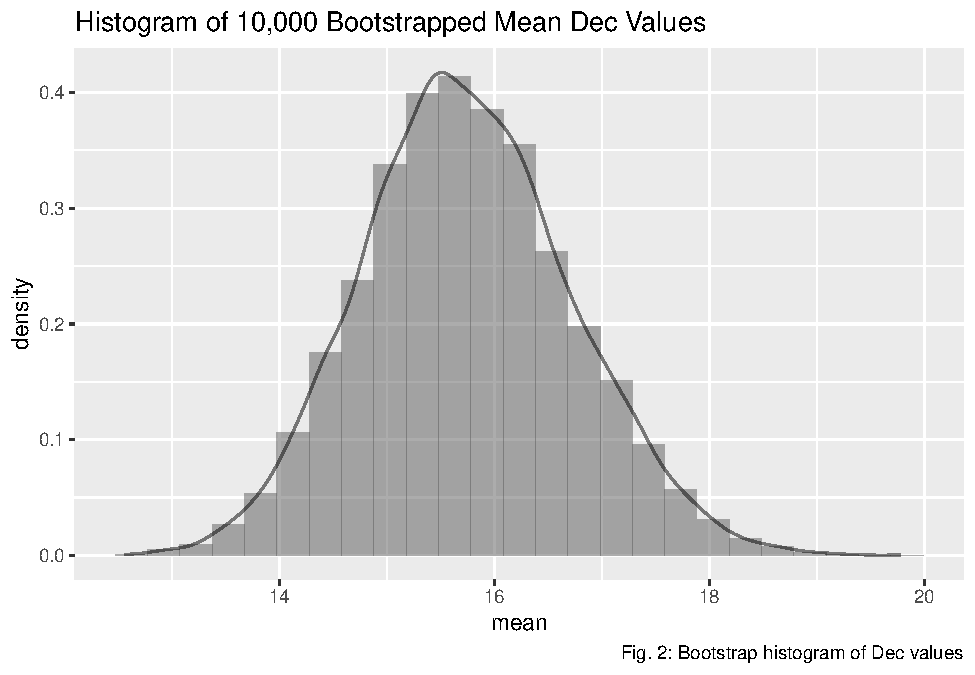
\includegraphics{paper_files/figure-latex/unnamed-chunk-1-1.pdf}

\hypertarget{standard-confidence-interval}{%
\subsection{Standard Confidence
Interval}\label{standard-confidence-interval}}

Confidence intervals are tools that are used to estimate a parameter.
Specifically, a confidence interval gives a range of values in which the
true value of the parameter may lie. An \(\alpha\)-level standard
confidence interval is given by
\[\hat{\theta}_S[\alpha] = \hat{\theta} \pm z_{\alpha}\hat{\sigma},\]
where \(\hat{\theta}\) is a point estimate of the parameter of interest
\(\theta\), \(\hat{\sigma}\) is the estimate of the standard deviation
of \(\hat{\theta}\) and \(z_{\alpha}\) is the \((100 *\alpha)\)th
percentile of the normal deviation \citep{Efron86}. We say that the
confidence interval constructed in this manner has a chance of capturing
the true parameter with a probability of \(\alpha\).

The standard confidence interval is built based on the assumption that
the distribution from which we are sampling is Normal. This means that
for an unknown distribution, the standard confidence interval could
present an incorrect range. However, the same process can be used with
bootstrap sampling to form the bootstrap percentile method. This means
that an approximate bootstrap confidence interval will be created in the
same automatic way that the standard confidence interval was created.
For bootstrapped confidence intervals, the number of bootstrap
replications \(B\) must be large (around 2000) due to the nature of
confidence intervals requiring greater accuracy \citep{Efron86}.

\hypertarget{the-percentile-method}{%
\subsection{The Percentile Method}\label{the-percentile-method}}

The percentile method interval is defined as the interval between the
\(100 * \alpha\) and the \(100(1 - \alpha)\) percentiles of the
bootstrap distribution of \(\hat{\theta}\). That is, the
\((1 - 2\alpha)\) coverage interval can be defined as
\([\hat{\theta}^*_\alpha,\hat{\theta}^*_{1-\alpha}]\)
\citep[\citet{EfronCasi}]{Efron86}. To go further, we can define
\(\hat{G}(t)\) as the bootstrap cdf, or the proportion of bootstrap
samples less than \(t\):
\[\hat{G}(t) = \frac{\#\{\hat{\theta^{*b} \leq t}\}}{B}.\] Thus the
\(\alpha\)th percentile point of the distribution is given by
\[\hat{\theta}_p[\alpha] = \hat{\theta^*_\alpha} = \hat{G}^{-1}(\alpha).\]
It follows that the percentile interval can be represented as
\[\left [ \hat{G}^{-1}(\alpha),\hat{G}^{-1}(1-\alpha) \right ].\] In the
case that the bootstrap distribution of
\(\hat{\theta}^* \sim N(\hat{\theta}, \hat{\sigma}^2)\), the
corresponding percentile interval would be equivalent to the standard
interval. However, this is not usually the case. When the bootstrap
distribution is non-normal, we can suppose that there exists, for all
\(\theta\), \[\hat{\phi} \sim N(\phi, \tau^2),\] for some monotone
transformation \(\hat{\phi} = g(\hat{\theta}), \phi = g(\theta)\), and
\(\tau\) is a constant. In other words, this transformation perfectly
normalizes the distribution of \(\hat{\theta}\). This transformation
invariant can be applied to the bootstrap replications such that
\[\hat{\phi}^{*b} = g\left( \hat{\theta}^{*b}\right ) \text{ for } b = 1,2,\dots, B.\]
The corresponding percentiles of the distribution transform similarly,
\(\hat{\phi}^*_\alpha = g \left ( \hat{\theta}^*_\alpha \right )\). Or
we can say that the \((1 - 2\alpha)\) percentile interval is
\(\hat{\phi} \pm \tau z_\alpha\) which can also be represented as
\([\hat{\phi}^*_\alpha,\hat{\phi}^*_{1-\alpha}]\). This means that the
interval on the \(\theta\) scale can be defined as
\[\hat{\theta}^*_\alpha = g^{-1}(\hat{\phi} \pm \tau z_\alpha).\] This
also can be represented as an interval,
\[\left [ g^{-1}(\hat{\phi} \pm \tau z_{1-\alpha}), g^{-1}(\hat{\phi} \pm \tau z_\alpha) \right ].\]
Therefore, the percentile method produces a correct interval for
\(\phi\) and due to the transformation invariance, also produces a
correct percentile interval for \(\theta\). This method assumes the
existence of some monotone normalizing mapping
\(\hat{\phi} = g(\hat{\theta}), \phi = g(\theta)\) and relies on that to
create a correct interval. Since the process is automatic, we do not
need to know the transformation itself, only that it exists. However, in
some cases, no monotone normalizing mapping will exist \citep{Efron86}.

\hypertarget{the-bias-corrected-bc-method}{%
\subsection{The Bias-Corrected (BC)
Method}\label{the-bias-corrected-bc-method}}

The next method we will be looking at is the bias-corrected percentile
method (BC method) which is an improvement upon the previous percentile
method because we now take into account the possibility of bias. It can
be shown that \(\hat{\theta}\) is biased upwards relative to \(\theta\)
which means that the confidence intervals should be adjusted downwards
\citep[\citet{EfronCasi}]{Efron86}. From our simulated bootstrap
replications
\(\hat{\theta}^{*1}, \hat{\theta}^{*2}, \dots ,\hat{\theta}^{*B},\)
define \[p_0 = \frac{\#\{\hat{\theta^{*b} \leq \theta}\}}{B},\] and
define the bias-correction value \[z_0 = \Phi^{-1}(p_0),\] where
\(\Phi^{-1}\) is the inverse function of the standard normal cdf. Thus
we define a transformation
\(\hat{\phi} = g(\hat{\theta)}, \phi = g(\theta)\) such that for any
\(\theta\), \[\hat{\phi} \sim N(\phi - z_0\tau, \tau^2),\] with \(z_0\)
and \(\tau\) constants. This means that we can say the bias corrected
method has an \(\alpha\)-level endpoint can be represented as
\[\hat{\theta}_{BC}[\alpha] = \hat{G}^{-1} \left [ \Phi \left ( 2z_0 + z_\alpha\right ) \right ].\]
If \(\hat{G} = 0.50\), then half of the bootstrap distribution is less
than \(\hat{\theta}\) and our bias-correction value \(z_0 = 0\). In this
case, the confidence interval produced by BC would be the same interval
produced by the percentile method.

\hypertarget{the-bias-corrected-and-accelerated-bca-method}{%
\subsection{The Bias-Corrected and Accelerated (BCa)
Method}\label{the-bias-corrected-and-accelerated-bca-method}}

A further modification upon the BC interval is the bias corrected and
accelerated method (BCa). For this method, we do not assume the the
standard error, \(\tau\) is constant as we did in the BC interval
\citep[\citet{EfronCasi}]{Efron86}. Rather, we assume the existence of a
monotone transformation
\(\hat{\phi} = g(\hat{\theta)}, \phi = g(\theta)\) such that for any
\(\theta\),
\[\hat{\phi} \sim N(\phi - z_0\tau_\phi, \tau_\phi^2) \text{ where } \tau_\phi = 1+ a\phi.\]
The \(a\) is known as the acceleration and is a constant that describes
how the standard deviation of \(\hat{\phi}\) varies with \(\phi\). In
other words, \(a\) is proportional to the skewness of the bootstrap
distribution. For example, for one-parameter exponential families,
\(a=z_0\), however, there are many different algorithms to compute and
estimate \(a\) \citep{Flowers18}. Now, our \(\alpha\)-level endpoint
from BCa is
\[\hat{\theta}_{BCa}[\alpha] = \hat{G}^{-1} \left [ \Phi \left ( z_0 + \frac{z_0+z_\alpha}{1-a(z_0+z_a)} \right ) \right ].\]
If \(a = 0\), then
\(\hat{\theta}_{BCa}[\alpha] = \hat{\theta}_{BC}[\alpha].\) When
calculating a BCa interval, the acceleration value \(a\) is not a
function of the bootstrap distribution and must be calculated
separately, however the process is algorithmic and can be calculated
without too much work. Each of the three previous methods (percentile,
BC, and BCa) all build upon each other and have less restrictive
assumptions, however computation increases as we loosen assumptions.

\hypertarget{the-bootstrap-t-studentized-method}{%
\subsection{The Bootstrap-t (Studentized)
Method}\label{the-bootstrap-t-studentized-method}}

The final method we explain is the bootstrap-t interval (or the
studentized method). Recall from earlier, our sample, \(X\) from which
we can calculate an estimate, \(\hat{\theta}(X)\) of the parameter of
interest \(\theta\) \citep[\citet{Puth15}]{Efron86}. We can also
estimate \(\hat{\sigma}(X)\) for the standard error of \(\theta\). We
can use these parameters to find the Student's \(t\)-statistic defined
as \[T = \frac{\hat{\theta} - \theta}{\hat{\sigma}}.\] As such, the
\(\alpha\)th percentile point of a confidence interval of \(\theta\)
would be \(\hat{\theta} - \hat{\sigma}T_{(\alpha)}\) where
\(T_{(\alpha)}\) represents the \(\alpha\)th percentile of the
\(t\)-distribution, \(T\). Unfortunately, the percentiles of the
t-distribution are unknown in most cases, but we can use bootstrapping
to estimate these percentiles. To do this, we perform a large number,
\(B\), of bootstrap samples, from which we can find the bootstrap
replications of the parameter of interest,
\(\hat{\theta^*} = \hat{\theta}(X^*)\), and the standard error,
\(\hat{\sigma^*} = \hat{\sigma}(X^*)\). From these we can calculate a
t-statistic for each bootstrap sample:
\[T^* = \frac{\hat{\theta}^* - \hat{\theta}}{\hat{\sigma}^*}.\] for each
bootstrap sample. Using a large number of these bootstrap samples, we
can estimate the percentiles of the \(t\)-distribution such that:
\[\hat{T}_{(\alpha)} = B*\alpha\text{th ordered value of all the bootstrap relications of }T^*.\]
This means that for \(B = 2000\) and \(\alpha = 0.90\), then
\(\hat{T}_{(\alpha)}\) is the 1,800th ordered point of all of the
bootstrap replications of \(T^*\). It follows that the \(\alpha\)th
studentized confidence interval endpoint can be given with
\[\hat{\theta}_T[\alpha] = \hat{\theta} - \hat{\sigma}T_{(\alpha)},\]
where we can estimate the standard error using
\[\hat{\sigma} = \frac{1-\hat{\theta}^2}{\sqrt{n}}.\] One of the main
factors why the studentized method is so popular is because we assume
that our bootstrapped statistic is pivotal which means that the
confidence interval does not depend on any other parameters. Instead, we
can calculate the appropriate confidence interval for the parameter of
interest specifically from the bootstrapped statistic
\citep[\citet{Puth15}]{Efron86}.

\hypertarget{simulation}{%
\section{Simulation}\label{simulation}}

Justin,

An example before a simulation could be useful if your simulation is
assessing their performance (i.e.~if your simulation is like Hmk 8,
where you do a lot of reps to check performance). You could run anything
on an existing data set (the one we have from Hmk 4/5), for example,
that you want. I think you have enough without worrying about the
parametric bootstrap.

\begin{Shaded}
\begin{Highlighting}[]
\FunctionTok{library}\NormalTok{(boot)}
\end{Highlighting}
\end{Shaded}

\begin{verbatim}
## 
## Attaching package: 'boot'
\end{verbatim}

\begin{verbatim}
## The following object is masked from 'package:mosaic':
## 
##     logit
\end{verbatim}

\begin{verbatim}
## The following object is masked from 'package:lattice':
## 
##     melanoma
\end{verbatim}

\begin{Shaded}
\begin{Highlighting}[]
\FunctionTok{set.seed}\NormalTok{(}\DecValTok{495}\NormalTok{)}

\NormalTok{reps }\OtherTok{\textless{}{-}} \DecValTok{2000}
\NormalTok{n }\OtherTok{\textless{}{-}} \DecValTok{50}

\NormalTok{X }\OtherTok{\textless{}{-}} \FunctionTok{rnorm}\NormalTok{(n, }\DecValTok{0}\NormalTok{, }\DecValTok{1}\NormalTok{)}
\NormalTok{values }\OtherTok{\textless{}{-}} \FunctionTok{data.frame}\NormalTok{(X)}

\NormalTok{mean.fun }\OtherTok{\textless{}{-}} \ControlFlowTok{function}\NormalTok{(d, i) \{}
\NormalTok{  d }\OtherTok{\textless{}{-}}\NormalTok{ X[i]}
  \FunctionTok{return}\NormalTok{ (}\FunctionTok{mean}\NormalTok{(d))}
\NormalTok{\}}

\NormalTok{results }\OtherTok{\textless{}{-}} \FunctionTok{boot}\NormalTok{(}\AttributeTok{data =}\NormalTok{ values, }\AttributeTok{statistic =}\NormalTok{ mean.fun, }\AttributeTok{R =}\NormalTok{ reps)}

\NormalTok{results}
\end{Highlighting}
\end{Shaded}

\begin{verbatim}
## 
## ORDINARY NONPARAMETRIC BOOTSTRAP
## 
## 
## Call:
## boot(data = values, statistic = mean.fun, R = reps)
## 
## 
## Bootstrap Statistics :
##        original       bias    std. error
## t1* 0.008974394 -0.003054148   0.1320787
\end{verbatim}

\begin{Shaded}
\begin{Highlighting}[]
\FunctionTok{plot}\NormalTok{(results)}
\end{Highlighting}
\end{Shaded}

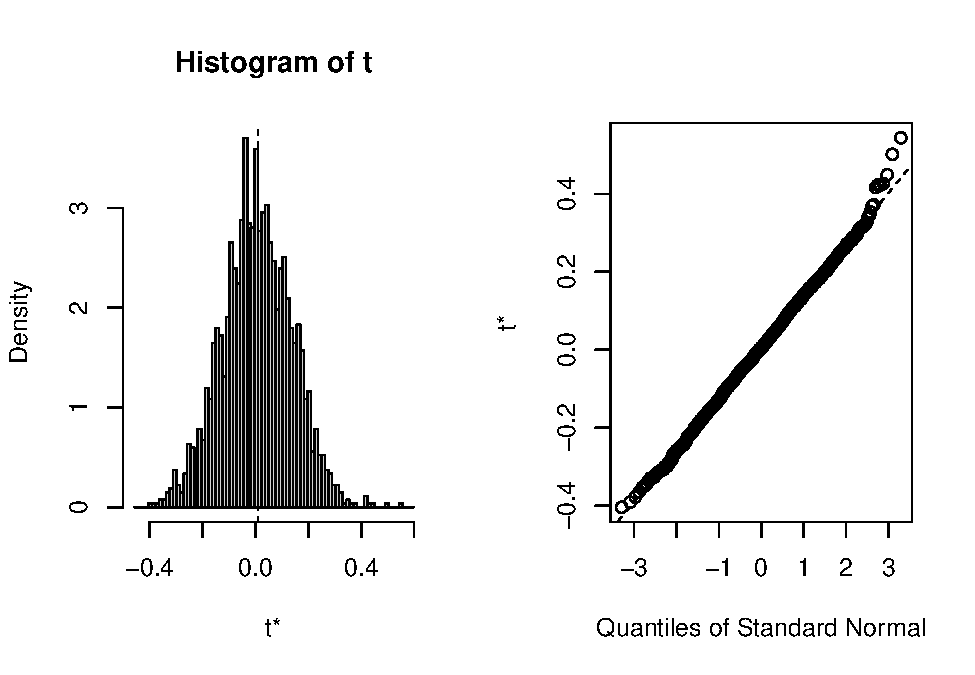
\includegraphics{paper_files/figure-latex/unnamed-chunk-2-1.pdf}

\begin{Shaded}
\begin{Highlighting}[]
\NormalTok{ci }\OtherTok{\textless{}{-}} \FunctionTok{boot.ci}\NormalTok{(results, }\AttributeTok{type =} \StringTok{"all"}\NormalTok{)}
\end{Highlighting}
\end{Shaded}

\begin{verbatim}
## Warning in boot.ci(results, type = "all"): bootstrap variances needed for
## studentized intervals
\end{verbatim}

\begin{Shaded}
\begin{Highlighting}[]
\FunctionTok{set.seed}\NormalTok{(}\DecValTok{1}\NormalTok{)}

\NormalTok{reps }\OtherTok{\textless{}{-}} \DecValTok{10000}
\NormalTok{n }\OtherTok{\textless{}{-}} \DecValTok{15}

\NormalTok{r\_pvals }\OtherTok{\textless{}{-}} \FunctionTok{rep}\NormalTok{(}\DecValTok{0}\NormalTok{, reps)}
\NormalTok{tau\_pvals }\OtherTok{\textless{}{-}} \FunctionTok{rep}\NormalTok{(}\DecValTok{0}\NormalTok{, reps)}

\ControlFlowTok{for}\NormalTok{(i }\ControlFlowTok{in} \DecValTok{1}\SpecialCharTok{:}\NormalTok{ reps) \{}
\NormalTok{  x }\OtherTok{\textless{}{-}} \FunctionTok{rnorm}\NormalTok{(n, }\DecValTok{40}\NormalTok{, }\DecValTok{3}\NormalTok{)}
\NormalTok{  y }\OtherTok{\textless{}{-}} \FunctionTok{rgamma}\NormalTok{(n, }\DecValTok{8}\NormalTok{, }\DecValTok{2}\NormalTok{)}
  
\NormalTok{  values }\OtherTok{\textless{}{-}} \FunctionTok{data.frame}\NormalTok{(x,y)}
  
\NormalTok{  r\_pvals[i] }\OtherTok{\textless{}{-}} \FunctionTok{with}\NormalTok{(values, }\FunctionTok{cor.test}\NormalTok{(x, y))}\SpecialCharTok{$}\NormalTok{p.value}
\NormalTok{  tau\_pvals[i] }\OtherTok{\textless{}{-}} \FunctionTok{with}\NormalTok{(values, }\FunctionTok{cor.test}\NormalTok{(x, y, }\AttributeTok{method =} \StringTok{"kendall"}\NormalTok{))}\SpecialCharTok{$}\NormalTok{p.value}
\NormalTok{\}}

\FunctionTok{sum}\NormalTok{(r\_pvals }\SpecialCharTok{\textless{}=} \FloatTok{0.05}\NormalTok{)}\SpecialCharTok{/}\NormalTok{reps}
\end{Highlighting}
\end{Shaded}

\begin{verbatim}
## [1] 0.0463
\end{verbatim}

\begin{Shaded}
\begin{Highlighting}[]
\FunctionTok{sum}\NormalTok{(tau\_pvals }\SpecialCharTok{\textless{}=} \FloatTok{0.05}\NormalTok{)}\SpecialCharTok{/}\NormalTok{reps}
\end{Highlighting}
\end{Shaded}

\begin{verbatim}
## [1] 0.0436
\end{verbatim}

\begin{Shaded}
\begin{Highlighting}[]
\NormalTok{simbootstraps }\OtherTok{\textless{}{-}} \ControlFlowTok{function}\NormalTok{(dataset, trueparameter) \{}
  
  
  
  \CommentTok{\# use the data set to create the bootstrapped distribution (1 bootstrap and then keep replicated statistic of interest)}
  \CommentTok{\# like 2000 times}
  
  \CommentTok{\#use that bootstrap distribution as follows to test for the intervals}
  
  \CommentTok{\# see how many times the true value lies inside the interval {-}{-}\textgreater{} first do one and then show the actual intervals}
  
\NormalTok{\}}



\NormalTok{simnormal }\OtherTok{\textless{}{-}} \ControlFlowTok{function}\NormalTok{(locationinput, scaleinput, testcenterinput, ninput, }\AttributeTok{repsinput =} \DecValTok{1000}\NormalTok{)\{}
\CommentTok{\# Set Useful Values}
\NormalTok{reps }\OtherTok{\textless{}{-}}\NormalTok{ repsinput }\CommentTok{\#number of repetitions}
\NormalTok{location }\OtherTok{\textless{}{-}}\NormalTok{ locationinput }
\NormalTok{scale }\OtherTok{\textless{}{-}}\NormalTok{ scaleinput}
\NormalTok{testcenter }\OtherTok{\textless{}{-}}\NormalTok{ testcenterinput }\CommentTok{\#center to test for}
\NormalTok{n }\OtherTok{\textless{}{-}}\NormalTok{ ninput }\CommentTok{\#sample size}

\CommentTok{\#Initialize storage vectors}
\NormalTok{tpvals }\OtherTok{\textless{}{-}} \FunctionTok{rep}\NormalTok{(}\DecValTok{0}\NormalTok{,reps)}
\NormalTok{spvals }\OtherTok{\textless{}{-}} \FunctionTok{rep}\NormalTok{(}\DecValTok{0}\NormalTok{,reps)}
\NormalTok{srpvals }\OtherTok{\textless{}{-}} \FunctionTok{rep}\NormalTok{(}\DecValTok{0}\NormalTok{,reps)}

\CommentTok{\#Generate random data, do tests, save p{-}values}
\ControlFlowTok{for}\NormalTok{(i }\ControlFlowTok{in} \DecValTok{1}\SpecialCharTok{:}\NormalTok{reps)\{}
\NormalTok{  x }\OtherTok{\textless{}{-}} \FunctionTok{rnorm}\NormalTok{(n, location, scale)}
\NormalTok{  tpvals[i] }\OtherTok{\textless{}{-}} \FunctionTok{t.test}\NormalTok{(}\SpecialCharTok{\textasciitilde{}}\NormalTok{x, }\AttributeTok{mu =}\NormalTok{ testcenter)}\SpecialCharTok{$}\NormalTok{p.value }
\NormalTok{  spvals[i] }\OtherTok{\textless{}{-}} \FunctionTok{SIGN.test}\NormalTok{(x, }\AttributeTok{md =}\NormalTok{ testcenter)}\SpecialCharTok{$}\NormalTok{p.value }
\NormalTok{  srpvals[i] }\OtherTok{\textless{}{-}} \FunctionTok{wilcox.test}\NormalTok{(x, }\AttributeTok{mu =}\NormalTok{ testcenter)}\SpecialCharTok{$}\NormalTok{p.value }
\NormalTok{\}}

\NormalTok{output }\OtherTok{\textless{}{-}} \FunctionTok{c}\NormalTok{(}\FunctionTok{sum}\NormalTok{(tpvals }\SpecialCharTok{\textless{}=} \FloatTok{0.05}\NormalTok{)}\SpecialCharTok{/}\NormalTok{reps, }\FunctionTok{sum}\NormalTok{(spvals }\SpecialCharTok{\textless{}=} \FloatTok{0.05}\NormalTok{)}\SpecialCharTok{/}\NormalTok{reps, }\FunctionTok{sum}\NormalTok{(srpvals }\SpecialCharTok{\textless{}=} \FloatTok{0.05}\NormalTok{)}\SpecialCharTok{/}\NormalTok{reps)}
\FunctionTok{names}\NormalTok{(output) }\OtherTok{\textless{}{-}} \FunctionTok{c}\NormalTok{(}\StringTok{"Ttest"}\NormalTok{, }\StringTok{"Sign"}\NormalTok{, }\StringTok{"SignedRank"}\NormalTok{)}
\NormalTok{output}
\NormalTok{\}}
\end{Highlighting}
\end{Shaded}

\begin{Shaded}
\begin{Highlighting}[]
\FunctionTok{set.seed}\NormalTok{(}\DecValTok{495}\NormalTok{)}

\NormalTok{reps }\OtherTok{\textless{}{-}} \DecValTok{10000}
\NormalTok{n }\OtherTok{\textless{}{-}} \DecValTok{15}

\NormalTok{r\_pvals }\OtherTok{\textless{}{-}} \FunctionTok{rep}\NormalTok{(}\DecValTok{0}\NormalTok{, reps)}
\NormalTok{tau\_pvals }\OtherTok{\textless{}{-}} \FunctionTok{rep}\NormalTok{(}\DecValTok{0}\NormalTok{, reps)}

\ControlFlowTok{for}\NormalTok{(i }\ControlFlowTok{in} \DecValTok{1}\SpecialCharTok{:}\NormalTok{ reps) \{}
\NormalTok{  y }\OtherTok{\textless{}{-}} \FunctionTok{rgamma}\NormalTok{(n, }\DecValTok{8}\NormalTok{, }\DecValTok{2}\NormalTok{)}
  
\NormalTok{  values }\OtherTok{\textless{}{-}} \FunctionTok{data.frame}\NormalTok{(x,y)}
  
\NormalTok{  r\_pvals[i] }\OtherTok{\textless{}{-}} \FunctionTok{with}\NormalTok{(values, }\FunctionTok{cor.test}\NormalTok{(x, y))}\SpecialCharTok{$}\NormalTok{p.value}
\NormalTok{  tau\_pvals[i] }\OtherTok{\textless{}{-}} \FunctionTok{with}\NormalTok{(values, }\FunctionTok{cor.test}\NormalTok{(x, y, }\AttributeTok{method =} \StringTok{"kendall"}\NormalTok{))}\SpecialCharTok{$}\NormalTok{p.value}
\NormalTok{\}}

\FunctionTok{sum}\NormalTok{(r\_pvals }\SpecialCharTok{\textless{}=} \FloatTok{0.05}\NormalTok{)}\SpecialCharTok{/}\NormalTok{reps}
\end{Highlighting}
\end{Shaded}

\begin{verbatim}
## [1] 0.0489
\end{verbatim}

\begin{Shaded}
\begin{Highlighting}[]
\FunctionTok{sum}\NormalTok{(tau\_pvals }\SpecialCharTok{\textless{}=} \FloatTok{0.05}\NormalTok{)}\SpecialCharTok{/}\NormalTok{reps}
\end{Highlighting}
\end{Shaded}

\begin{verbatim}
## [1] 0.0456
\end{verbatim}

\bibliographystyle{agsm}
\bibliography{bibliography.bib}


\end{document}
